\subsection{Kinematics}
\label{sec:geometrical_analysis}

\paragraph{Massive activations.}
In both ConvNeXt models one stage-3 channel exceeds all others by more than an order
of magnitude (channel $236$ tied, $195$ untied), and in Swin the four corner tokens
do~\citep{sun2024massiveactivationslargelanguage,darcet2024vision}; ResNet shows no
such outlier.
The network relies on the ConvNeXt channel (zeroing it in the tied model costs
$\massiveZeroCost$ points, a random channel at most $\randomChannelCost$), but it would
dominate every geometric statistic, so we remove it from all measurements and leave the
forward pass unchanged (\cref{app:massive-activations}).

\paragraph{Kinematics.}
On refined trajectories ($R{=}100$, $\Delta t{=}0.01$, $N{=}500$) we measure the speed
$\|v\|$, the angular velocity $\omega$ of the heading $\hat v$, the split of the
acceleration into a tangential part $a_t=\langle\hat v,a\rangle$ and a normal part
$a_n$ and the curvature $\kappa=a_n/\|v\|^2$
(\cref{fig:kinematics-compare,tab:kinematics}).
Curvature is read against the arc travelled per unit of depth,
$s\approx\|v\|\Delta t$: the heading turns by
$\Delta\theta\approx\kappa\|v\|\Delta t$ (equivalently $\omega\Delta t$).
A value $\kappa\sim 10^{-2}$ with $\|v\|$ of tens still turns the heading by tens of
degrees over a block.
Earlier work measures turning angles between consecutive layers or
frames~\citep{henaff2019perceptual,hosseini2023straighten,pandey2026trajectorygeometrytransformerrepresentations};
refinement gives them within a block.

\begin{figure*}[t]
    \centering
    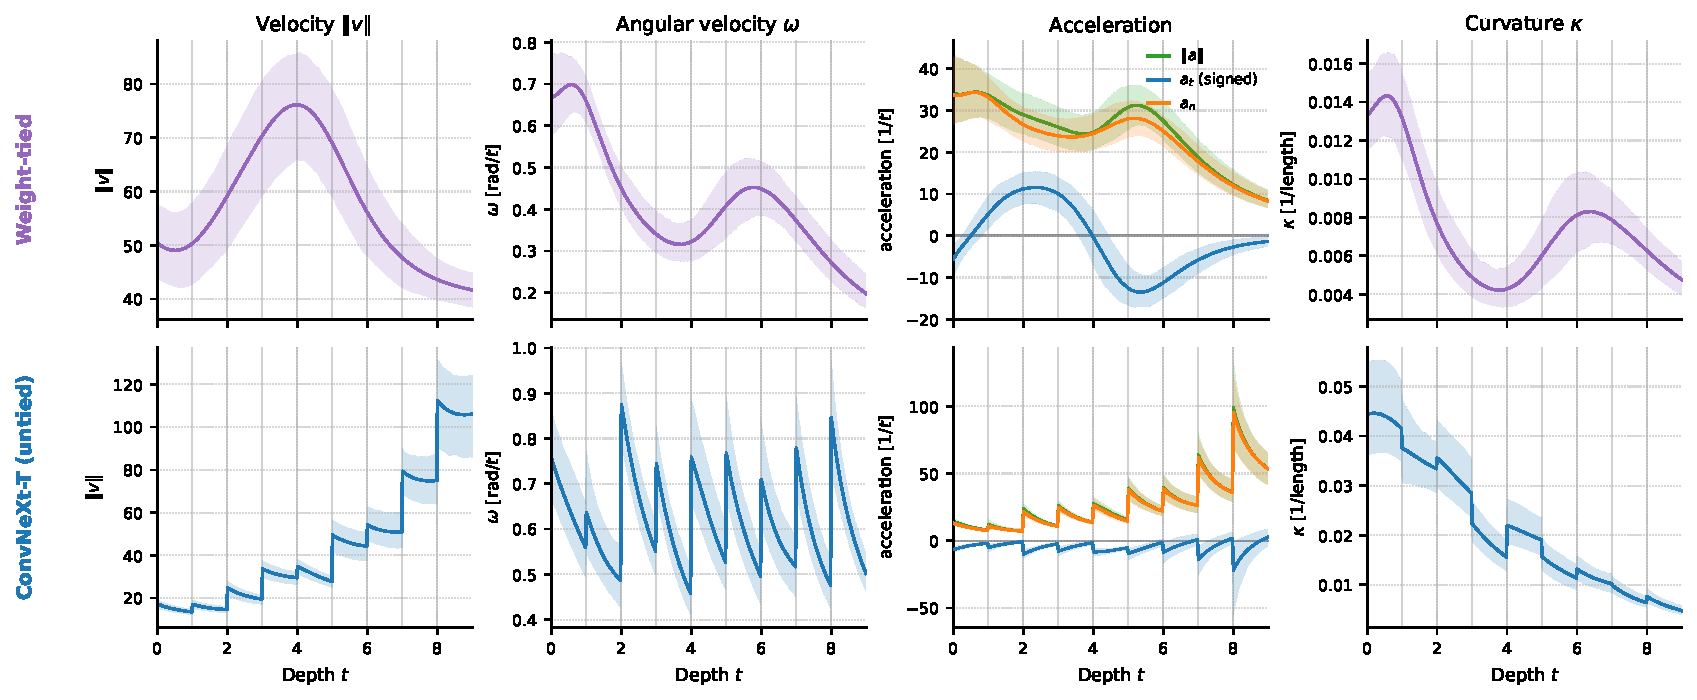
\includegraphics[width=\textwidth]{figures/kinematics_compare.pdf}
    \caption{Stage-3 kinematics over $T{=}9$ ($R{=}100$, Euler $\Delta t{=}0.01$;
    massive channel removed; mean and P5--P95 over $N{=}500$).
    \textbf{Top:} weight-tied ConvNeXt.
    \textbf{Bottom:} untied ConvNeXt-T.
    Columns: speed $\|v\|$, angular velocity $\omega$, acceleration
    $(\|a\|,a_t,a_n)$, curvature $\kappa{=}a_n/\|v\|^2$.
    On the untied row, pairs of micro-steps that straddle a block boundary are omitted
    from $\omega$, $a$ and $\kappa$: there $v$ is discontinuous and finite differences
    diverge as $\Delta t\!\to\!0$.}
    \label{fig:kinematics-compare}
\end{figure*}

\begin{table}[t]
    \centering
    \caption{Stage-3 kinematics ($R{=}100$, $N{=}500$, massive channel removed).
    Untied values inside blocks; sign flips: share of coordinates of $v$ that change
    sign across one micro-step.}
    \label{tab:kinematics}
    \small
    \setlength{\tabcolsep}{3pt}
    \resizebox{\linewidth}{!}{%
    \begin{tabular}{lcc}
        \toprule
        & Tied & Untied \\
        \midrule
        $\|v\|$                 & peak $76.2$ at $t{=}3.98$ & $14.8\to112.5$ in steps \\
        $\omega$ (rad$/t$)      & peak $0.70$ at $t{=}0.58$ & $0.64$--$0.87\to0.46$--$0.56$ \\
        $\kappa$ ($10^{-3}$)    & $14.3$, min $4.2$ at $t{=}3.79$ & $44.4$ (block 0), $6.0$ (block 8) \\
        $a_n/\|a\|$             & $0.95$ & $0.97$ \\
        $\|a\|$, first$\to$last & $34.3\to8.4$ & $14.5\to53.5$ \\
        turn at boundary        & -- & $\turnLow$--$\turnHigh^\circ$ \\
        sign flips, switch      & -- & $\signFlipBoundary\%$ \\
        sign flips, inside      & $\signFlipInsideTied\%$ & $\signFlipInsideUntied\%$ \\
        \bottomrule
    \end{tabular}%
    }
\end{table}

\paragraph{The tied stage searches, expands and refines.}
The shared field traces one arc in three phases (\cref{fig:kinematics-compare}, top).
Early on the speed is moderate while $\omega$ and $\kappa$ peak
($0.70\,\mathrm{rad}/t$ at $t{=}0.58$), so the heading turns by about $40^\circ$ per
unit of depth: small steps that keep changing direction.
The tangential acceleration then turns positive, peaks at $t{=}2.34$ and crosses zero
at $t{=}3.98$, where the speed peaks; $\kappa$ reaches its minimum just before
($4.2{\times}10^{-3}$ at $t{=}3.79$, about $18^\circ$ per unit of depth).
The tangent still carries $28\%$ of $\|a\|$, a large share in a $75{,}000$-dimensional
state, but $a_n$ never vanishes.
After mid-horizon the field brakes ($a_t$ is most negative at $t{=}5.35$), the speed
falls and $\omega$ rebounds near $t{=}5.8$.
At $t{=}9$ the speed is still $41.7$ with $\omega{=}0.20$: the state is coasting, not
at a fixed point, which is consistent with the collapse when the integration continues
past $T$ (\cref{sec:usable-limit}).

\paragraph{The untied stage is a switched staircase.}
The untied ConvNeXt-T has no such arc (\cref{fig:kinematics-compare}, bottom).
At each integer the next block replaces the field and the heading jumps by
$\turnLow^\circ$ to $\turnHigh^\circ$ ($\turnMean^\circ$ on average) in a single
micro-step.
The large $\omega$ spikes at those boundaries are not turns of a hundred radians:
they are $\arccos\langle\hat v_d,\hat v_{d+1}\rangle/\Delta t$ on one micro-step of
$\Delta t{=}0.01$, so the heading jump is $\omega\Delta t\approx
\omegaDtTurnLow$--$\omegaDtTurnHigh\,\mathrm{rad}$
($\turnLow^\circ$--$\turnHigh^\circ$).
Dividing a finite angle by a vanishing step is why the spikes explode; they only record
that neighbouring blocks do not share a direction.
At the switch, $\signFlipBoundary\%$ of the coordinates of $v$ change sign, against
$\signFlipInsideUntied\%$ per micro-step inside a block and $\signFlipInsideTied\%$ in
the tied model, which has no boundaries.
Inside a block the motion is short: $\omega$ starts at $0.64$--$0.87$ and settles at
$0.46$--$0.56$, and $\kappa$ falls from $4.4{\times}10^{-2}$ in the first block to
$6.0{\times}10^{-3}$ in the last as the speed grows.
The speed envelope rises in steps, from $14.8$ in the first block to $112.5$ at the
start of the last, with no stage-wide acceleration and braking.
The path is therefore a chain of nine shallow arcs joined by near-orthogonal turns;
\cref{sec:nine-directions} measures how these pieces add up.
